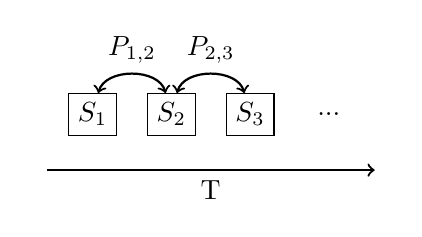
\begin{tikzpicture}
    \node[draw,rectangle] (a) {$S_1$};
    \node[draw,rectangle,right of=a] (b) {$S_2$};
    \node[draw,rectangle,right of=b] (c) {$S_3$};
    \node[rectangle,right of=c] (d) {...};

    \node[rectangle,below left of=a] (A) {};
    \node[rectangle,below right of=d] (D) {};
    \draw[thick,->] (A) edge node[below] {T} (D);

    \draw[thick,<->] (a) edge[out=75,in=105] node[above] {$P_{1,2}$} (b);
    \draw[thick,<->] (b) edge[out=75,in=105] node[above] {$P_{2,3}$} (c);
    %~ \draw[thick,<->] (c) edge[out=80,in=100] node[above] {$P_{..}$} (d);
\end{tikzpicture}
